\documentclass{beamer}
\usetheme{metropolis}           % Use metropolis theme
\title{Modelling heat diffusion from magnetic nanoparticles to the surrounding tissue}
\date{\today}
\author{James Brisbourne}
\institute{University of York}
\begin{document}
  \maketitle
  
  
  \section{Magnetic Hyperthermia}
  
  
  
  
  \begin{frame}{What is magnetic hyperthermia}
  \begin{itemize}
  \item Type of thermal cancer treatment that takes advantage of the heat generated by magnetic nanoparticles
  \item Mangetic nanoparticles can trasnform electromagnetic energy into heat
  \end{itemize}
  
	\begin{figure}
	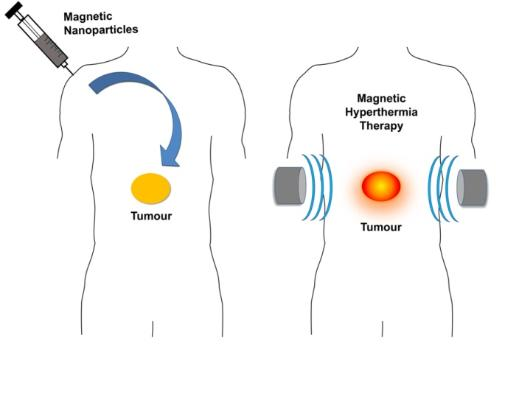
\includegraphics[scale=0.4]{injection.jpg}
\end{figure}	  
  
  \end{frame}

  \begin{frame}[shrink=10]{Pennes' Bioheat Equation}
  
\begin{itemize}
\item Used as a standard model for predicting temperature distributions in living tissue for over 50 years
\end{itemize}
  
\begin{equation}
\rho c \frac{\partial T}{\partial t} =  k \left( \frac{\partial ^2 T}{\partial x^2} + \frac{\partial ^2 T}{\partial y^2} + \frac{\partial ^2 T}{\partial z^2} \right) + \rho _{blood} c_{blood} w(T_{a} - T) + Q_{met} + Q_i(x,y,z,t)
\end{equation}  
$\rho$ is the density of the tissue
\newline
$c$ is the specific heat capacity of the tissue  
\newline
$k$ is the tissue thermal conductivity
\newline
$T$ is the local tissue temperature
\newline
$T_a$ is the arterial blood temperature
\newline
$\omega$ is the local tissue-blood perfusion rate
\newline
$Q_{met}$ tissue metabolic rate
  
  
  \end{frame}
  
  
  
  
  \begin{frame}{Pennes' Bioheat Equation Shortcomings}
  
\begin{itemize}
\item Thermal equilibrium doesn't occur in the capillaries, as Pennes assumed
\item Doesn't take into account the directionality of blood perfusion between vessels and tissue
\item Basically doesn't account for some of the significant features of the circulatory system
\end{itemize}
  
  \end{frame}
  




	\begin{frame}{1D Heat Diffusion Model}
Simplified the equation to 1 dimension to make the problem easier:

\begin{equation}
\frac{\partial T}{\partial t} =  \frac{k}{\rho c} \frac{\partial ^2 T}{\partial x^2} +  \frac{\rho _{blood} c_{blood}w}{\rho c}(T_{a} - T) + Q_{met} + Q_i(x,t)
\end{equation}

\begin{equation}
\frac{\partial T}{\partial t} =  a \frac{\partial ^2 T}{\partial x^2} +  C_1(T_{a} - T) + C_2(x,t) + C_3
\end{equation}

We now arrive at the simplest possible equation for the system:

\begin{equation}
\frac{\partial T(x,t)}{\partial t} =  a \frac{\partial ^2 T(x,t)}{\partial x^2}
\end{equation}


	\end{frame}
	
	\begin{frame}{Testing the model}
	Input function:
	\begin{equation}
	f_0 = \sin \left( \frac{\pi x}{L} \right)
	\end{equation}
	Analytic solution to this:
	
	\begin{equation}
	f(x,t) = \sin \left( \frac{\pi x }{L} \right) \exp \left( - \frac{\alpha \pi ^2 t}{L^2} \right) 
	\end{equation}
	\end{frame}
	
	\begin{frame}
	\begin{figure}
	\centering
	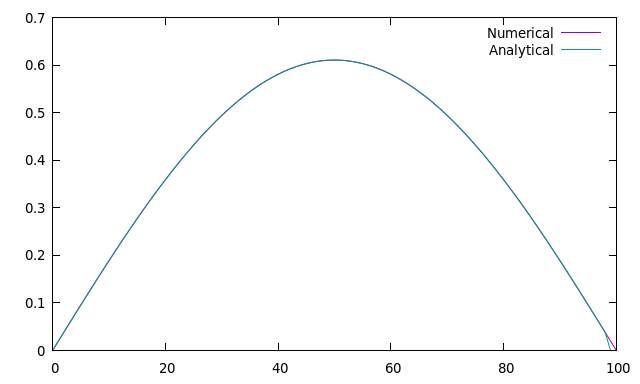
\includegraphics[scale=0.5]{1.png}
	\caption{dt = 0.00005, dx = 0.01, N = 100, runs = 1000, time = 0.05}
\end{figure}
	\end{frame}
	
	\begin{frame}
	\begin{figure}
	\centering
	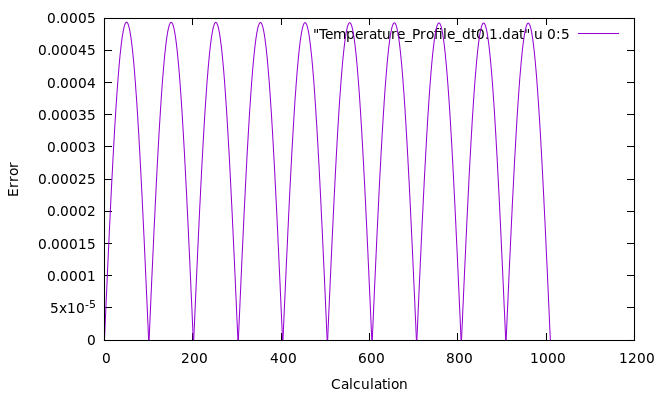
\includegraphics[scale=0.5]{2.png}
\end{figure}
	\end{frame}
	
	\begin{frame}
	\begin{figure}
	\centering
	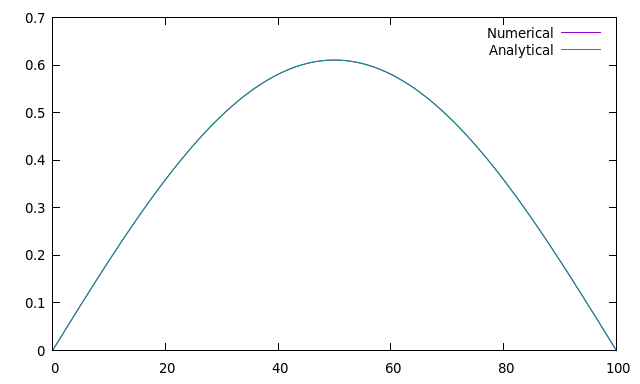
\includegraphics[scale=0.5]{3.png}
	\caption{dt = 0.00005, dx = 0.01, N = 100, runs = 1000, time = 0.05}
\end{figure}
	\end{frame}
	
	\begin{frame}
	\begin{figure}
	\centering
	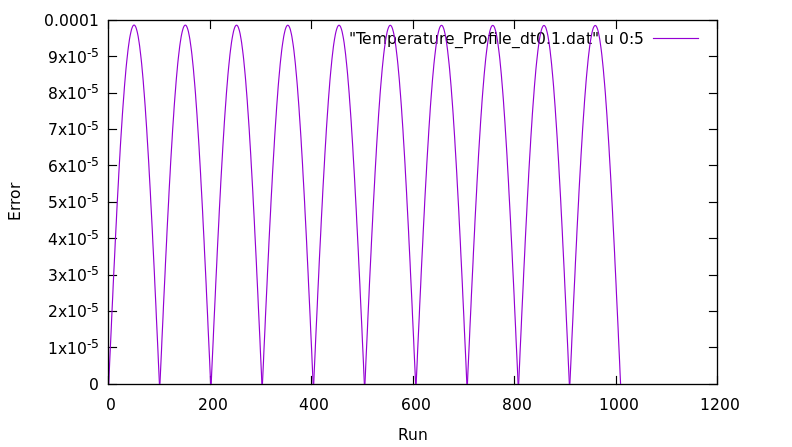
\includegraphics[scale=0.4]{4.png}
\end{figure}
	\end{frame}
	
	\begin{frame}
	\begin{figure}
	\centering
	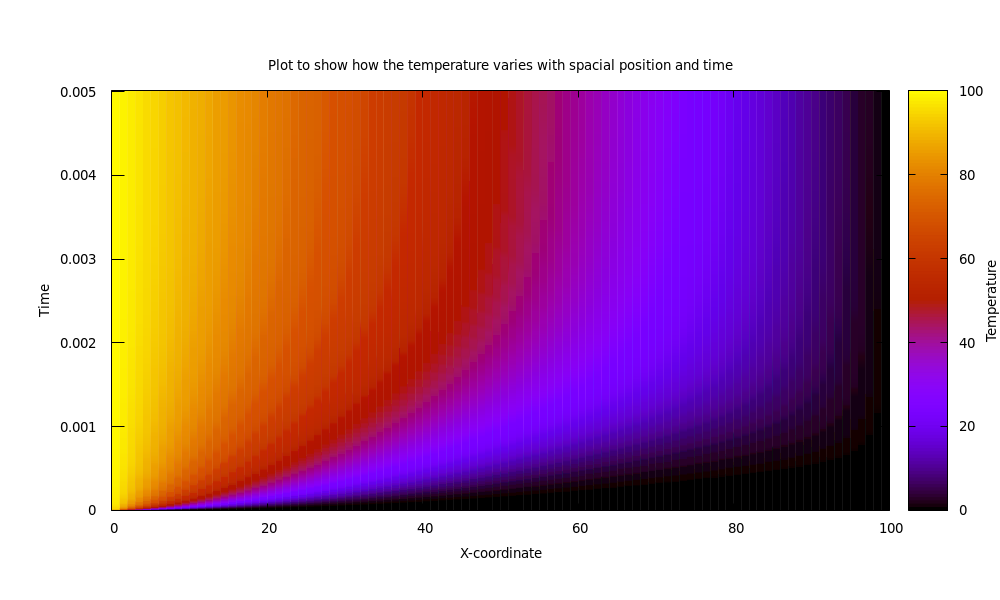
\includegraphics[scale=0.32]{5.png}
	\caption{dt = 0.0000001, dx = 0.001, runs = 50000, time = 0.005}
\end{figure}
	\end{frame}
	
		
	\begin{frame}
	\begin{figure}
	\centering
	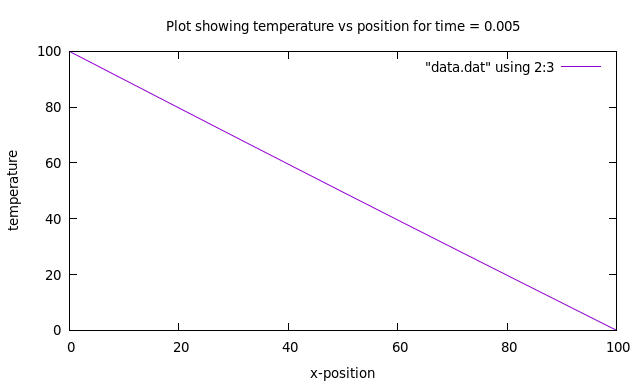
\includegraphics[scale=0.52]{6.png}
\end{figure}
	\end{frame}
	
	\begin{frame}
	Heat capactity of magnetite can be described by the Shomate equation:
	\begin{equation}
    C_p = A + BT + CT^2 + DT^3 + \frac{E}{T^2}
\end{equation}
For temperatures $298K - 900K$:
$$A = 104.2096,\; B = 178.5108,\; C = 10.61510,\; D = 1.132534,$$ \\ $$ E = -0.994202 $$
For temperatures $900K - 3000K$:
$$A = 200.8320,\; B = 1.586435 \times 10^{-7},\; C = -6.661682 \times 10^{-8},$$\\ $$ D = 9.452452 \times 10^{-9},\; E = 3.186020 \times 10^{-8}$$ \url{https://webbook.nist.gov/cgi/cbook.cgi?ID=C1309382&Mask=2&Type=JANAFS&Plot=on}
	\end{frame}
\end{document}
